\begin{frame}[t]{Cleaning Algorithms}
    \raisebox{10ex}{
    \begin{overlayarea}{0.36\textwidth}{3.5cm}
      \only<1>{
      \begin{itemize}
        \setlength\itemsep{1em}
        \item \code{white}{TailcutsImageCleaner}
        \item \code{white}{MARSImageCleaner}
        \item \code{white}{FACTImageCleaner}
        \item \code{white}{TimeConstrainedImageCleaner}
      \end{itemize}
      }
      \only<2>{
      \begin{itemize}
        \setlength\itemsep{1em}
        \item \code{white}{TailcutsImageCleaner}
        \item \code{white!50!black}{MARSImageCleaner}
        \item \code{white!50!black}{FACTImageCleaner}
        \item \code{white!50!black}{TimeConstrainedImageCleaner}
      \end{itemize}
      }
      \only<3>{
      \begin{itemize}
        \setlength\itemsep{1em}
        \item \code{white!50!black}{TailcutsImageCleaner}
        \item \code{white}{MARSImageCleaner}
        \item \code{white!50!black}{FACTImageCleaner}
        \item \code{white!50!black}{TimeConstrainedImageCleaner}
      \end{itemize}
      }
      \only<4>{
      \begin{itemize}
        \setlength\itemsep{1em}
        \item \code{white!50!black}{TailcutsImageCleaner}
        \item \code{white!50!black}{MARSImageCleaner}
        \item \code{white}{FACTImageCleaner}
        \item \code{white!50!black}{TimeConstrainedImageCleaner}
      \end{itemize}
      }
      \only<5>{
      \begin{itemize}
        \setlength\itemsep{1em}
        \item \code{white!50!black}{TailcutsImageCleaner}
        \item \code{white!50!black}{MARSImageCleaner}
        \item \code{white!50!black}{FACTImageCleaner}
        \item \code{white}{TimeConstrainedImageCleaner}
      \end{itemize}
      }
    \end{overlayarea}
    }
    \raisebox{10ex}{
    \begin{overlayarea}{0.58\textwidth}{3.5cm}
      \only<2>{
      \begin{itemize}%TailcutsImageCleaner
        \item [•] Selects pixels that pass a \code{white!70!black}{picture} and \code{white!70!black}{boundary threshold}
        \item [•] Most basic implementation of the cleaning algorithms
      \end{itemize}
      }
      \only<3>{
      \begin{itemize}%MARSImageCleaner
        \item [•] Selects pixels that pass a \code{white!70!black}{picture} and \code{white!70!black}{boundary threshold}, analogous to \code{white!70!black}{TailcutsImageCleaner}
        \item [•] Also selects pixels that are a neighbor of a neighbor of a core pixel, if they are above the \code{white!70!black}{boundary threshold}
      \end{itemize}
      }
      \only<4>{
      \begin{enumerate}%FACTImageCleaner
        \item Finds all pixels that contain more photons than the \code{white!70!black}{picture threshold}
        \item Removes pixels with less than \(N\) neighbors
        \item Adds remaining neighbors that are above the \code{white!70!black}{boundary threshold}
        \item Removes pixels that have less than \(N\) neighbors, that arrive within a given timeframe
        \item Removes pixels that have less than \(N\) neighbors
        \item Removes pixels that have less than \(N\) neighbors, arriving within a given timeframe
      \end{enumerate}
      }
      \only<5>{
      \begin{enumerate}%TimeConstrainedImageCleaner
        \item Finds all core pixels above the \code{white!70!black}{picture threshold}
        \item Removes pixels with less than \(N\) neighbors
        \item Removes all pixels that arrive within a time limit of the average arrival time
        \item Finds all neighbboring pixels above the \code{white!70!black}{boundary threshold}
        \item Removes all pixels with less than \(N\) neighbors arriving within a given timeframe
      \end{enumerate}
      }
    \end{overlayarea}
    }
    \only<2>{
      \centering
      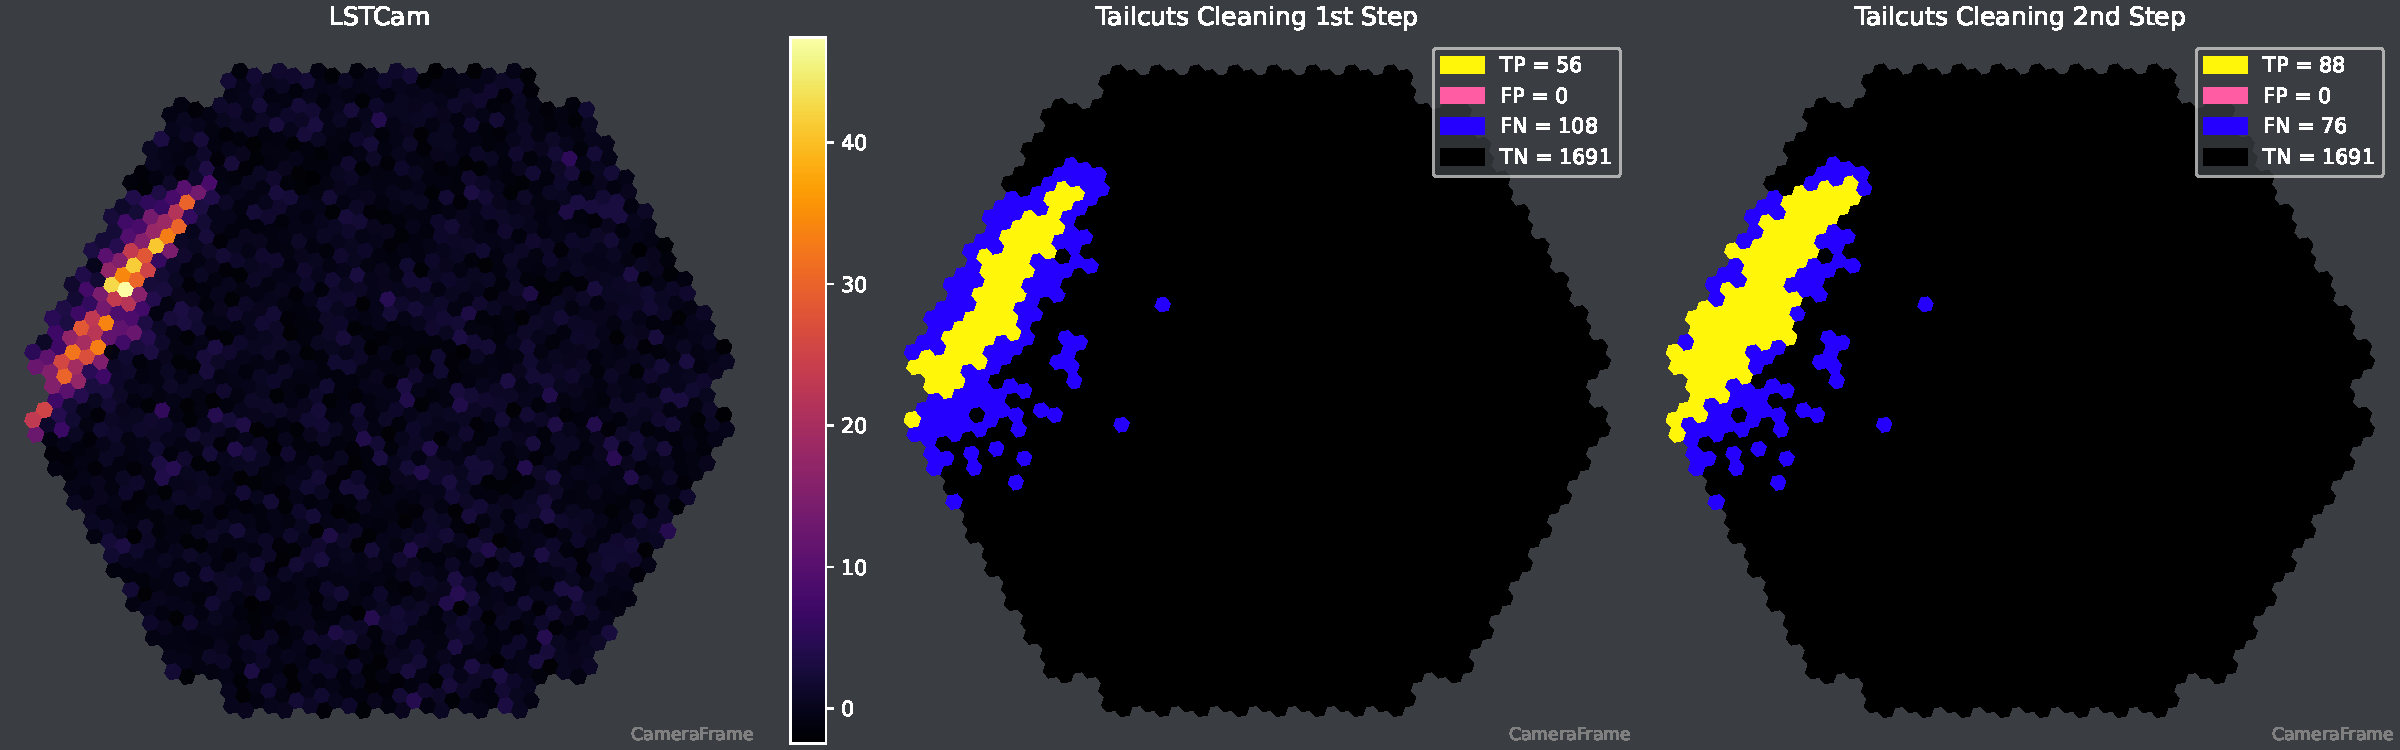
\includegraphics[height=0.15\textwidth]{plots/dl1_plots/run990_999_Tailcuts_event_463.pdf}
    }
    \only<3>{
      \centering
      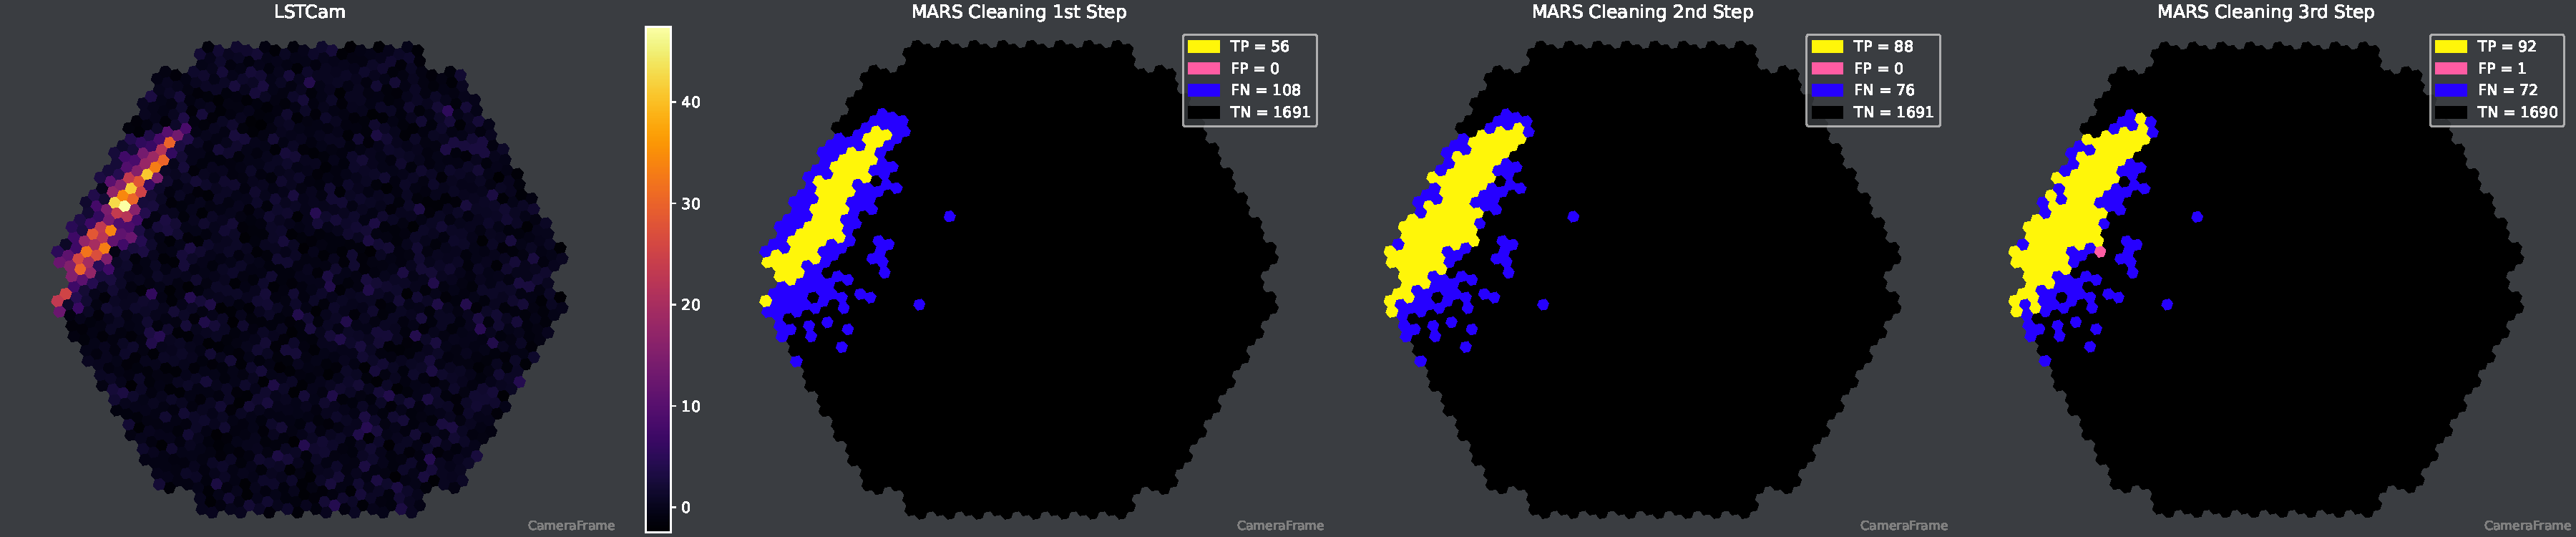
\includegraphics[height=0.15\textwidth]{plots/dl1_plots/run990_999_MARS_event_463.pdf}
    }
    \only<4>{
      \centering
      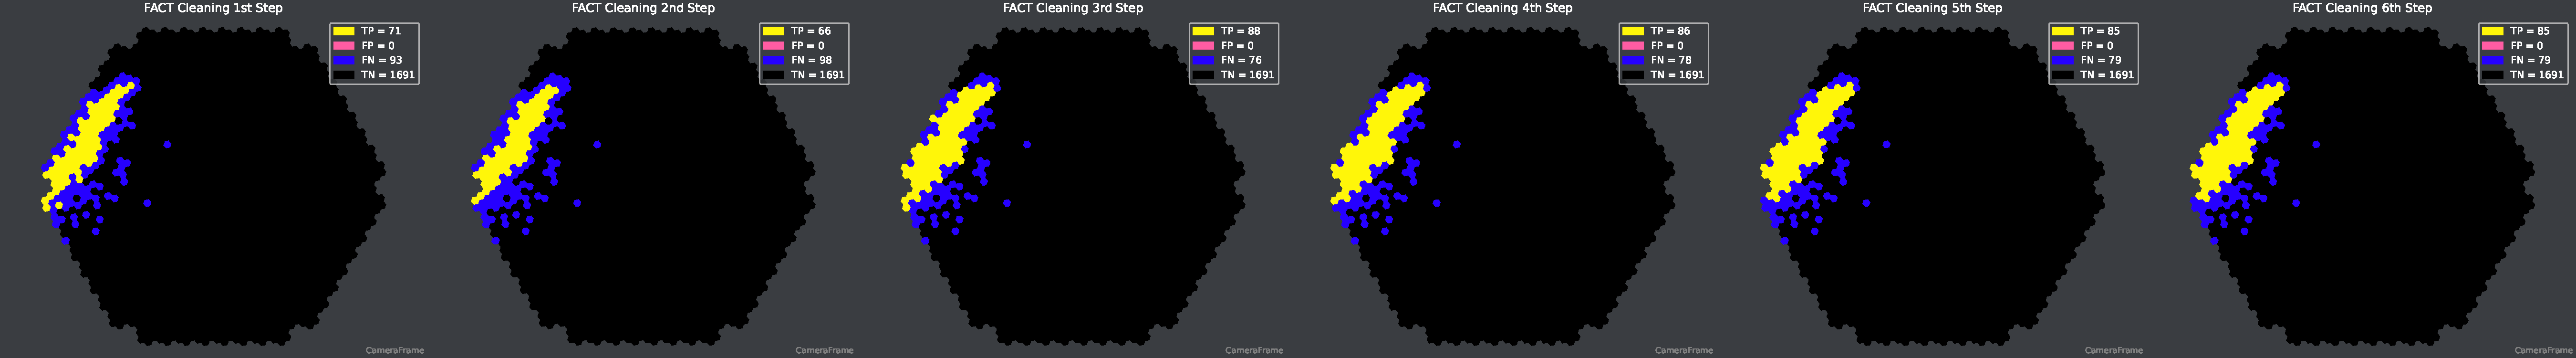
\includegraphics[height=0.13\textwidth]{plots/dl1_plots/run990_999_FACT_event_463.pdf}
    }
    \only<5>{
      \centering
      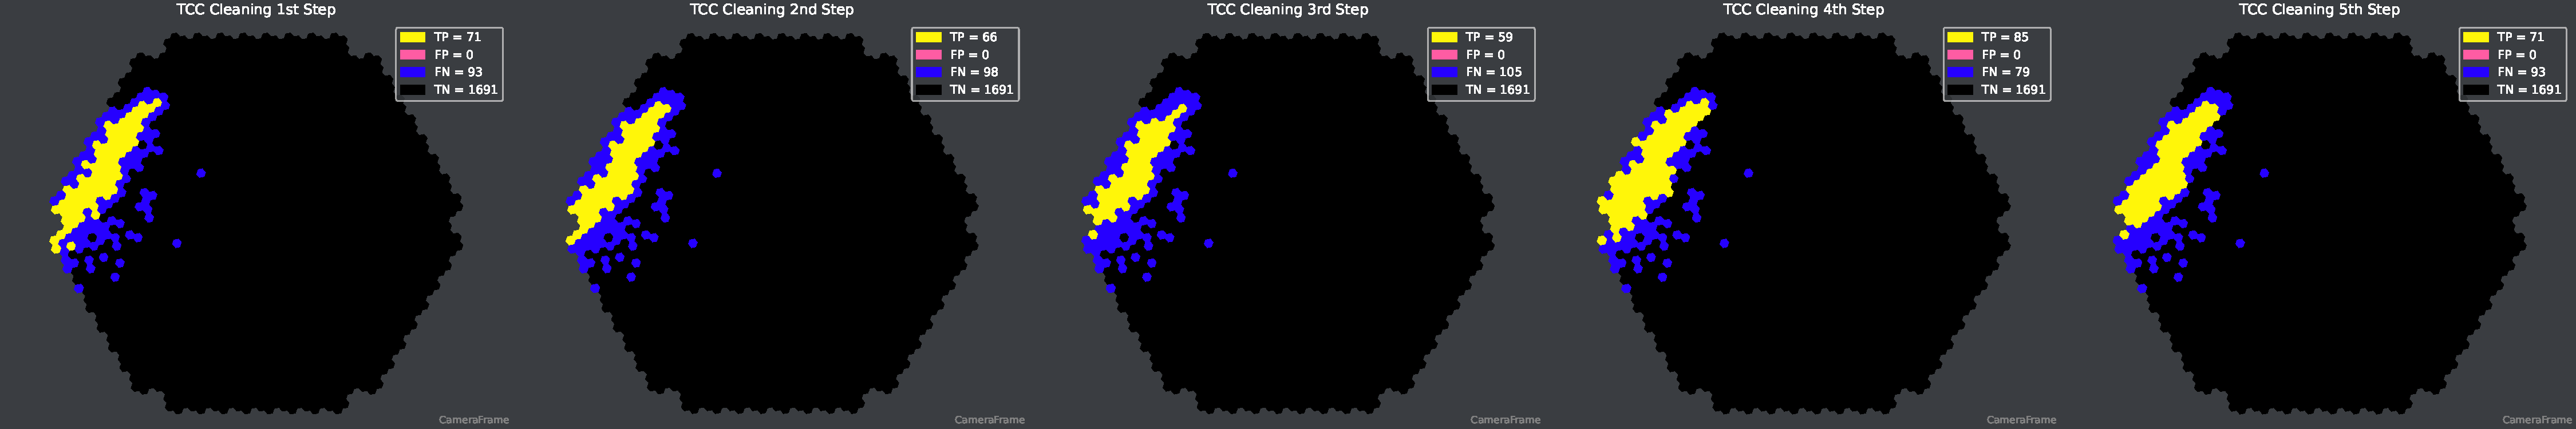
\includegraphics[height=0.15\textwidth]{plots/dl1_plots/run990_999_TCC_event_463.pdf}
    }
  \end{frame}